

Neben den geplanten Messungen zur Bestimmung der Schirmdämpfung der vorliegenden Proben sollen in diesem Abschnitt ebenfalls Messungen bezüglich einiger Feldeigenschaften innerhalb der Messkammer ausgewertet werden. Anschließend wird auf die ersten Einfügungsmessungen eingegangen und verschiedene Anpassungen vorgestellt, die zur Verbesserung der Signalqualität vorgenommen wurden. Die Gegenüberstellung der finalen Messungen mit den Werten der Vergleichsmessung erfolgt abschließend zur Verifikation des Teststandes.
\par
\vspace{\linespace}
Die Befestigung des Reflektors auf dem dafür vorgesehenen Holzstativ war einer der letzten Schritte des Aufbaus. Die Wirkung auf das Übertragungsverhalten zwischen den Antennen kann anhand der folgenden \Abb\ref{fig:4_Vergleich_Reflektor} nachvollzogen werden.
\par
\vspace{\linespace}


\begin{figure}[ht]
    \centering
    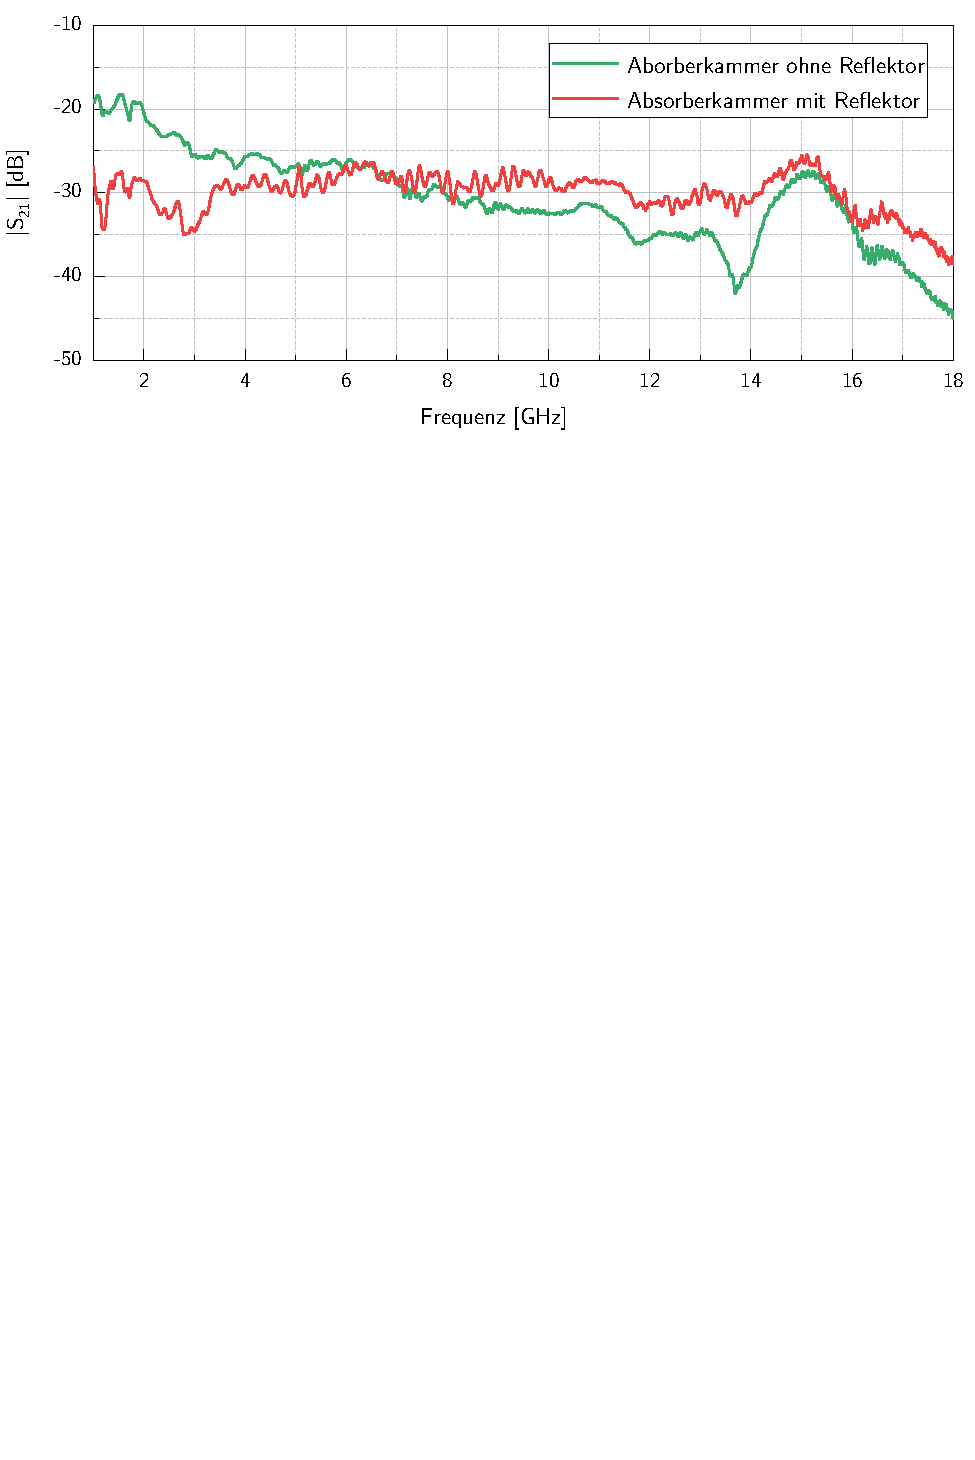
\includegraphics[page=1, width = .99\textwidth, trim = 0cm 17.4cm 0cm 0cm, clip]{Abbildungen/Kapitel4/Messergebnisse/Vergleich mit und ohne Reflektor (geerdet).pdf}
    \caption{Gemessener Transmissionskoeffizient ohne und mit eingebautem Reflektor}
    \label{fig:4_Vergleich_Reflektor}
\end{figure}

Zu erkennen ist, dass es aufgrund der Größe des Reflektorfensters vor allem im unteren Frequenzbereich zu einer erhöhten Dämpfung der Transmission kommt, was unter anderem auf die Wirkung der Öffnung als Blende zurückzuführen ist. Eine ähnliche Wirkung kann auch beim Einfügen des Probenhalters beobachtet werden, dessen Öffnung noch etwas kleiner ist. Die Geometrien der Öffnungen wurden, wie bereits im \Kapitel\ref{cha:3} erwähnt, unter anderem aufgrund der Größe der vorhandenen und zukünftigen Proben in dieser Art gewählt. Eine weitere mögliche Erklärung wäre, dass durch den Reflektor ein großer Teil der indirekten Strahlengänge über den Boden der Kammer blockiert wird, die andernfalls zu einer Verstärkung, gegenüber einer ideal absorbierenden Bodenplatte, an der Empfangsantenne führen. 
\par
\vspace{\linespace}
Die Verringerung der Freiraumdämpfung durch Einfügen des Reflektors im oberen Frequenzbereich kann wahrscheinlich auf konstruktive Interferenz mit den zusätzlich reflektierten Wellenfronten zurückgeführt werden. Abgesehen von den auftretenden kurzfrequenten Schwankungen im Signal der Freiraumdämpfung mit Reflektor ist die Charakteristik und Größenordnung jedoch ebenfalls mit der Referenzmessung vergleichbar.
\par
\vspace{\linespace}
Das Einfügen des Probenhalters in die vorgesehene Halterung verändert die Charakteristik der Freiraumdämpfung nur geringfügig bis auf eine ausgezeichnete Dämpfung bei ca. \SI{1,13}{\giga\hertz} mit einem Gütefaktor

\begin{equation}
    Q = \frac{f}{B}
    %f0 = 1,1296; fL = 1,12783M; fH = 1,13151; mit -66,2252 Peaktiefe
\end{equation}

von $Q \approx 307$ (vgl. \Abb\ref{fig:4_Vergleich_Probenhalter}). Zu beachten ist hier, dass Signale unterhalb der kritischen Frequenz von $f_k \approx 1,498\;\si{\giga\hertz}$ nach \Tabelle\ref{tab:2_Grenzwellenlaengen_Hohlleiter} mit der Öffnung des Probenhalters von $a = 10\;\si{\centi\meter}$ ohnehin eine starke Dämpfung erfahren, sodass Messungen unterhalb von etwa \SI{2}{\giga\hertz} mit dem durch die Anforderungsliste vorgegebenen Messausschnitt nur unter Vorbehalt durchzuführen sind. Dies wird durch die beobachtete Dämpfung bei etwas über \SI{1}{\giga\hertz} bestätigt, welche die Charakteristik der Freiraumdämpfung im Frequenzbereich zwischen \SI{0.8}{\giga\hertz} und \SI{1.6}{\giga\hertz} stark beeinflusst. %Erklärung --> Beugung oder so
\par
\vspace{\linespace}

\begin{figure}[ht]
    \centering
    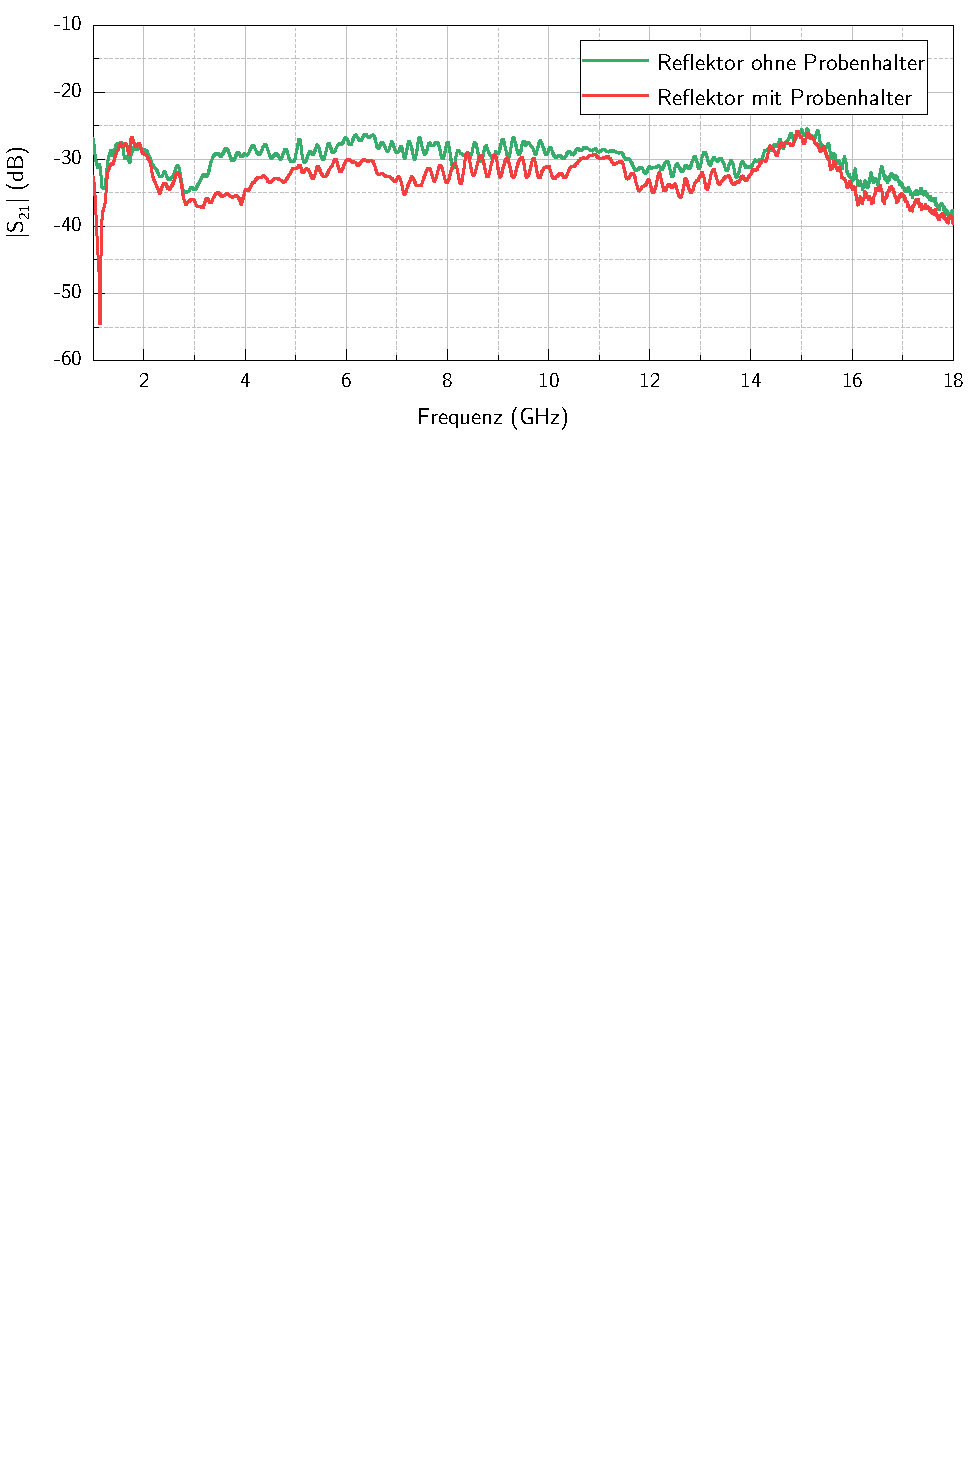
\includegraphics[page=1, width = .99\textwidth, trim = 0cm 17.4cm 0cm 0cm, clip]{Abbildungen/Kapitel4/Messergebnisse/Vergleich mit und ohne Probenhalter (geerdet).pdf}
    \caption{Gemessener Transmissionskoeffizient ohne und mit eingebautem Probenhalter}
    \label{fig:4_Vergleich_Probenhalter}
\end{figure}


Eine mögliche Erklärung, warum es abgesehen von der erwarteten Dämpfung aufgrund des Messausschnittes zu einem ausgezeichneten negativen Peak des gemessenen Transmissionskoeffizienten mit einem relativ hohen Gütefaktor kommt, könnte die Beugung der Wellen an der Öffnung des Probenhalters sein, welche das Signal von der Sendeantenne aufgrund der Abmessungen vor allem bei der beobachteten Frequenz von ca. \SI{1,13}{\giga\hertz} besonders stark beeinflusst. Dies würde erklären, warum eine so starke Dämpfung bei der Messung ohne Probenhalter, und wie sich im Folgenden zeigen wird auch bei Messungen mit Proben, welche die Öffnung bis auf kleine Spalte schließen, nicht zu beobachten ist. Dies kann jedoch nur vermutet werden, da in Bezug darauf keine näheren Untersuchungen durchgeführt wurden. 
\par
\vspace{\linespace}
Weiterhin wurde der Einfluss der Bodenplatte auf die Transmission untersucht. Dabei wurde auf Grundlage der Untersuchungen in~\cite{Vergleich_Absorberhalle_Groundplane} ein Vergleich zwischen reflektierendem Boden und einem mit Absorbern ausgelegten indirekten Koppelpfad unterhalb des Reflektors durchgeführt. Das Ziel der Betrachtung war, ebenso wie in~\cite{Vergleich_Absorberhalle_Groundplane}, festzustellen, inwieweit die Messungen durch die Interaktion mit vom Boden reflektierten Wellenanteilen beeinflusst werden. Die Messwerte und die Differenz beider Verläufe sind in der \Abb\ref{fig:4_Vergleich_Absorber_unter_Reflektor} dargestellt.
\par
\vspace{\linespace}

\begin{figure}[ht]
    \centering
    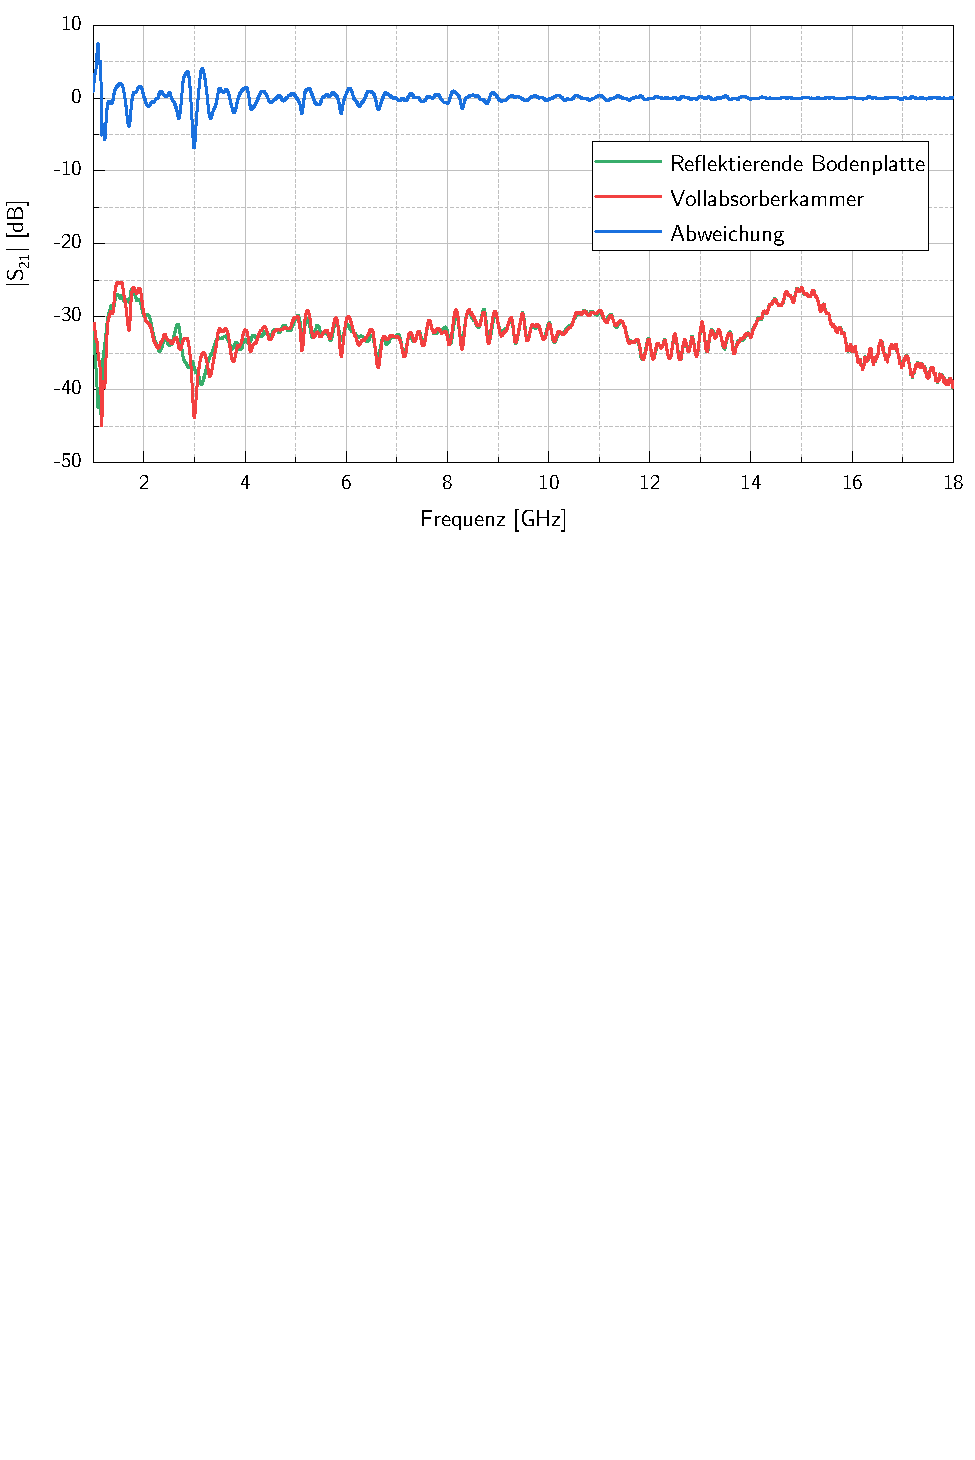
\includegraphics[page=1, width=.99\textwidth, trim = 0cm 15.6cm 0cm 0cm]{Abbildungen/Kapitel4/Messergebnisse/Vergleich Absorber unter Reflektor.pdf}
    \caption{Vergleichmessung der Transmission mit reflektierender und absorbierender Bodenplatte}
    \label{fig:4_Vergleich_Absorber_unter_Reflektor}
\end{figure}


Zu erkennen ist, dass der Einfluss wie erwartet vor allem in den unteren Frequenzbereichen mit Amplituden zwischen \SI{5}{\Dezibel} und \SI{10}{\Dezibel} am größten ist. Da jedoch auch oberhalb von \SI{4}{\giga\hertz} ein nicht zu vernachlässigender Einfluss zu erkennen ist, ist die Platzierung von Absorbern, vor allem direkt unterhalb des Reflektors, zur Verbesserung der Signalqualität durchaus zu empfehlen. Alle anderen Messungen wurden deshalb, wie auch im Abschnitt~\ref{cha:3_sub_Konstruktion} beschrieben, mit einer möglichst vollständig durch Absorber bedeckten Bodenplatte, insbesondere im Bereich der Antennenstative und unterhalb des Reflektors, durchgeführt.
\par
\vspace{\linespace}
Da die bereits vorhandenen Stative der Antennen vollständig aus Aluminium bestehen, sollte deren Einfluss auf die Messungen ebenfalls untersucht werden. Dazu wurden die Stative sende- und empfangsseitig mit je einem Pyramidenabsorber bedeckt und eine Vergleichsmessung nur mit eingebautem Reflektor ohne Probenhalter durchgeführt. Das Ergebnis ist in \Abb\ref{fig:4_Vergleich_Absorber_vor_Stativen} ersichtlicht.
\par
\vspace{\linespace}


\begin{figure}[ht]
    \centering
    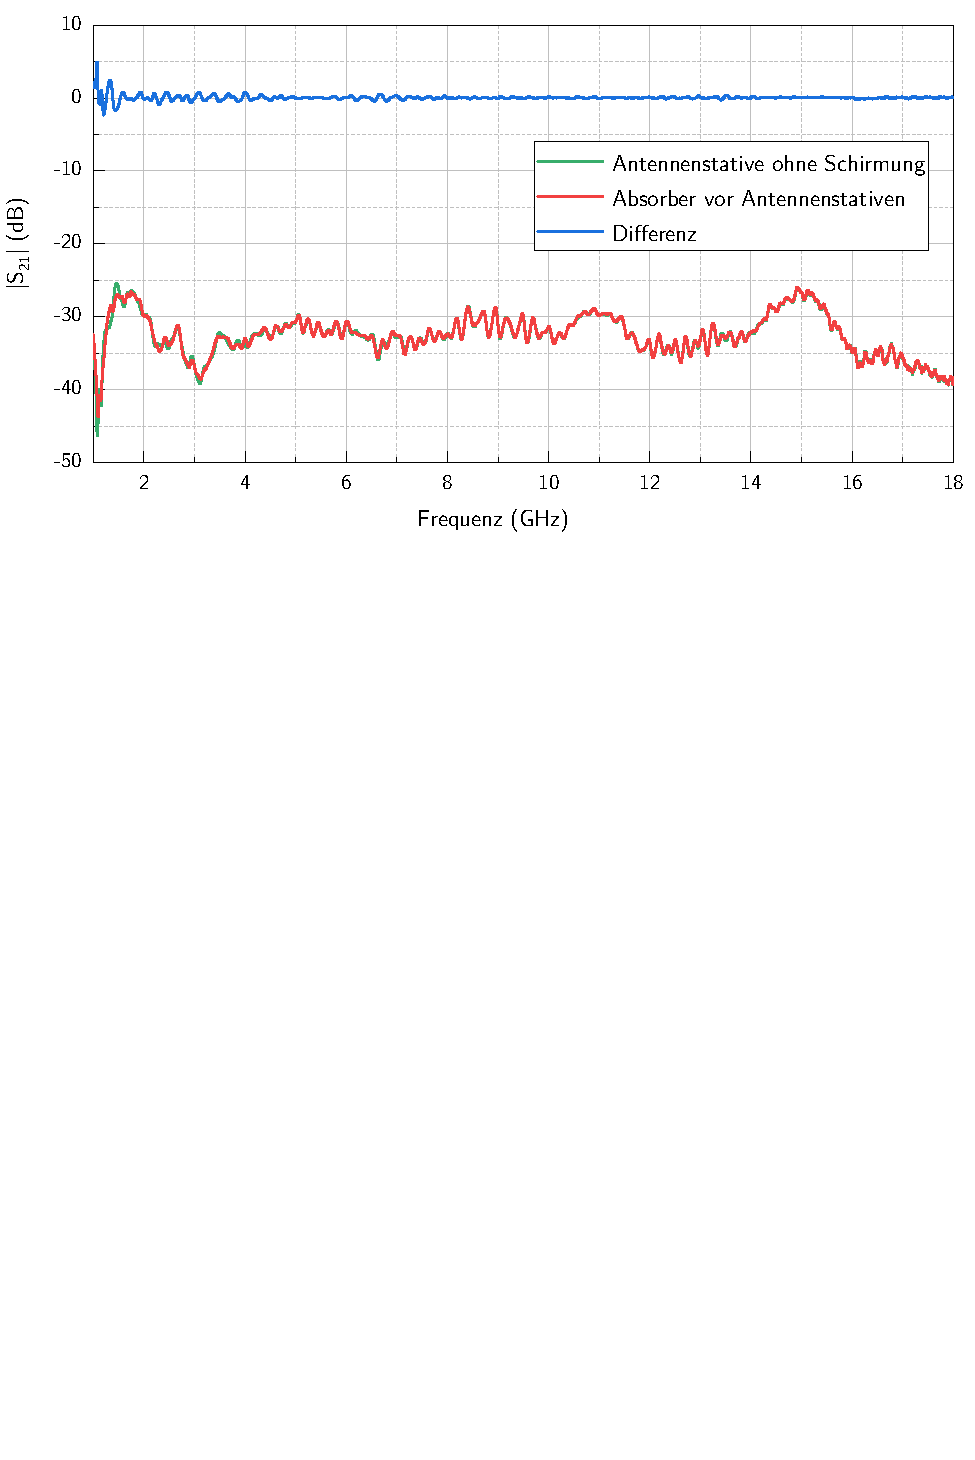
\includegraphics[page=1, width=.99\textwidth, trim = 0cm 15.6cm 0cm 0cm]{Abbildungen/Kapitel4/Messergebnisse/Vergleich Absorber vor Antennenstativen.pdf}
    \caption{Vergleichsmessung der Transmission mit unbedeckten und geschirmten Stativen}
    \label{fig:4_Vergleich_Absorber_vor_Stativen}
\end{figure}


Die zu beobachtende Differenz beider Vergleichsmessungen ist wesentlich geringer als der Einfluss von platzierten Absorbern unterhalb des Reflektors und beschränkt sich im Wesentlichen auf Frequenzen unterhalb von 2 bis \SI{4}{\giga\hertz}. Da die Maße der meisten stabförmigen Bestandteile der Stative die Wellenlänge des Messsignals bei \SI{4}{\giga\hertz} überschreiten, findet oberhalb dieser Frequenz keine Beeinflussung aufgrund dessen statt, dass Teile des Stativs als Stabantenne wirken. Da auch die Vergleichsmessungen für die geplanten Versuche oberhalb von \SI{4}{\giga\hertz} durchgeführt wurden, wurde die Abdeckung der Antennenstative anhand der vorliegenden Vergleichsmessung als eine der sekundären Maßnahmen zur Verbesserung der Signalqualität gegenüber anderen eingeordnet, die im Folgenden vorgestellt werden.
\par
\vspace{\linespace}
In \Abb\ref{fig:4_erste_Messung} ist das Ergebnis der ersten mit dem Aufbau durchgeführten Schirmdämpfungsmessung der Probe $9,5\times9,5-1$ dargestellt. Die Ermittlung der Schirmdämpfung aus den Messwerten der Freiraumdämpfung und der Dämpfung mit Probe wurde in \Abschnitt\ref{cha:4_Allgemeines} beschrieben. Die Bezeichung der Probe bezieht sich auf die Balkenlänge und -breite der in die Leiterplatte eingebrachten kreuzförmigen Muster, welche in \Abb\ref{fig:4_Probenhalter_mit_Probe} zu sehen sind.
\par
\vspace{\linespace}


\begin{figure}[ht]
    \centering
    \includegraphics[page = 4, width = .99\textwidth, trim = 0cm 14.3cm 0cm 0cm, clip]{Abbildungen/Kapitel4/Messergebnisse/9k5x9k5-1.pdf}
    \caption{Erste Schirmdämpfungsmessung der Probe $9,5\times9,5-1$}
    \label{fig:4_erste_Messung}
\end{figure}


Zu erkennen ist der durch die Bearbeitung der leitfähigen Schicht der Leiterplatte hervorgerufene Bandpass im Bereich zwischen \SI{9}{\giga\hertz} und \SI{10}{\giga\hertz}. Weiterhin ist jedoch auch der Effekt der bereits beschrieben Dämpfung bei etwa über \SI{1}{\giga\hertz} bei Messung der Freiraumdämpfung mit leerem Probenhalter zu erkennen, der sich aufgrund der Subtraktion von den Messwerten mit Probe in einer scheinbaren Verstärkung im Verlauf der Schirmdämpfung äußert. Da dieser Effekt wie bereits beschrieben auf die Größe des Messausschnittes zurückführbar zu sein scheint, soll im Weiteren darauf nicht näher eingegangen werden. 
\par
\vspace{\linespace}
Es ist außerdem ersichtlich, dass die ermittelte Schirmdämpfung im Bereich des Bandpasses und vor allem bei hohen Frequenzen teilweise stark fluktuiert. Um die Ursache hierfür zu ermitteln und die Qualität der Messung zusätzlich zu verbessern wurden die nachfolgenden Anpassungen, deren Ergebnisse in den \Abbildungen\ref{fig:4_9k5x9k5-1_Erdung}, \ref{fig:4_9k5x9k5-1_Absorberplatzierung} und \ref{fig:4_9k5x9k5-1_Schrauben} ersichtlich sind, vorgenommen. Anzumerken ist, dass alle abgebildeten Messsignale stabil waren und sich auch über mehrere Scandurchläufe, abgesehen vom statistischen Rauschen, nicht veränderten. Weiterhin wurden alle Konnektoren bezüglich einer korrekten Verschraubung überprüft, sodass dies als Ursache für die Fluktuationen auszuschließen ist. Die Kalibration des VNA wurde ebenfalls wie in \Abschnitt\ref{cha:4_Kalibration_Messtechnik} beschrieben durchgeführt. 
\par
\newpage
Die zusätzliche Erdung des Reflektors durch Verbindung mit der geerdeten äußeren Schirmhülle der Testkammer hat einen positiven Einfluss über dem gesamten Frequenzbereich (vgl. \Abb\ref{fig:4_9k5x9k5-1_Erdung}). Entsprechend der durchgeführten Versuche war dabei die Verbindung mit der Wand des Messkabine ausreichend für die Verbesserung, auch wenn letztere nicht mit dem Erdpotenzial verbunden war.  
\par
\vspace{\linespace}

\begin{figure}[H]
    \centering
    \includegraphics[page = 2, width = .99\textwidth, trim = 0cm 15.6cm 0cm 0cm, clip]{Abbildungen/Kapitel4/Messergebnisse/9k5x9k5-1.pdf}
    \caption[Vergleich des Einflusses der Erdung auf die Messwerte]{Vergleich des Einflusses der Erdung auf die Messwerte für \mbox{$9,5\times9,5-1$}}
    \label{fig:4_9k5x9k5-1_Erdung}
\end{figure}

\begin{figure}[ht]
    \centering
    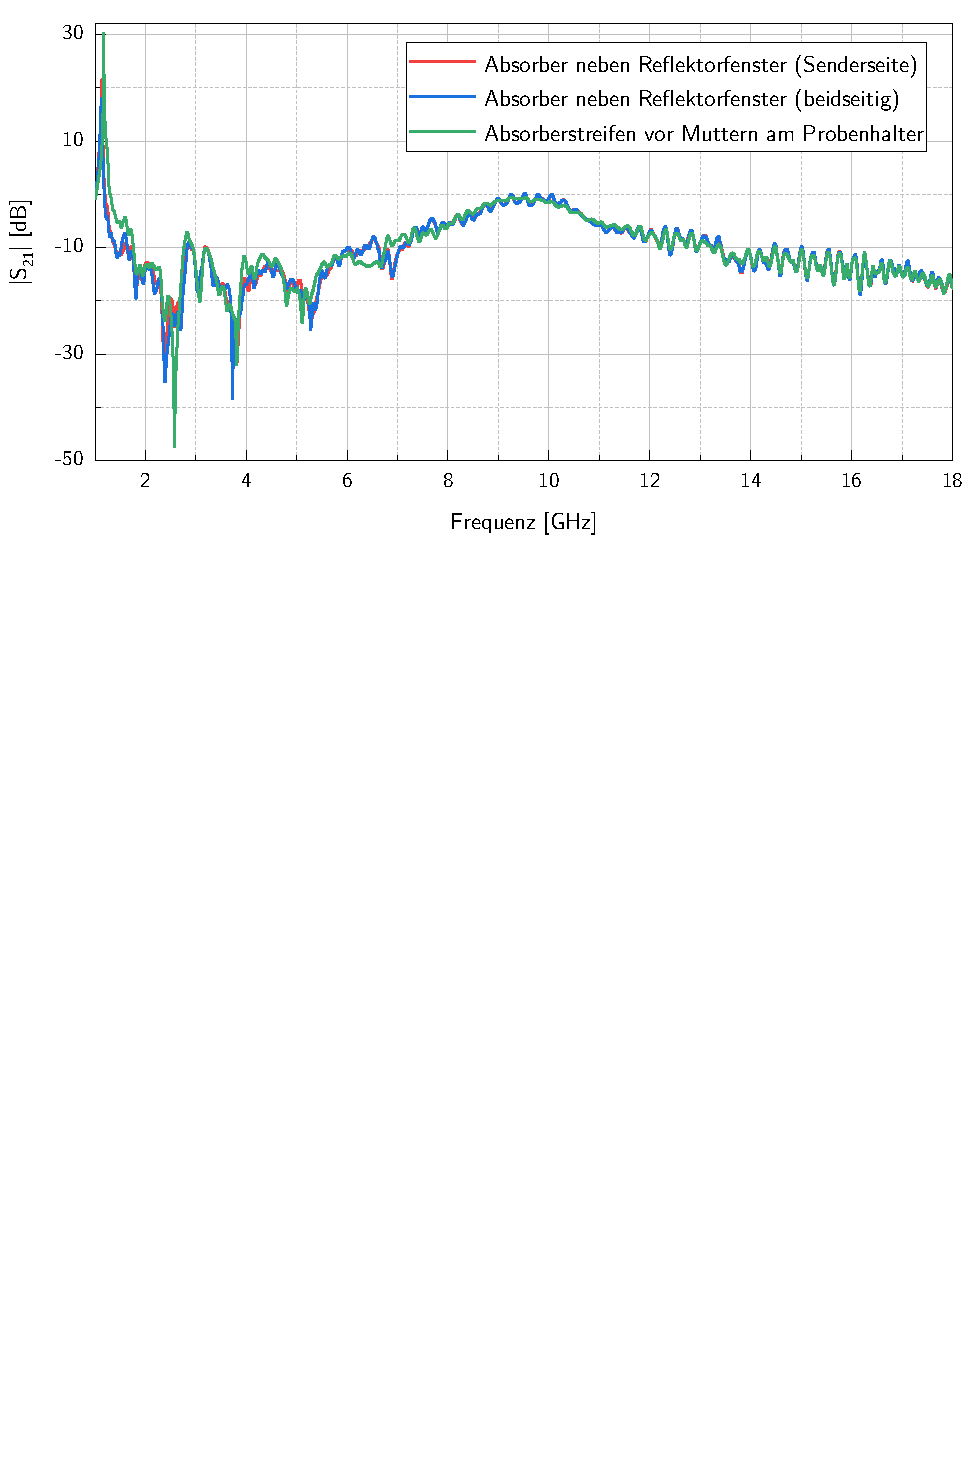
\includegraphics[page = 1, width = .99\textwidth, trim = 0cm 14.3cm 0cm 0cm, clip]{Abbildungen/Kapitel4/Messergebnisse/9k5x9k5-1.pdf}
    \caption[Vergleich des Einflusses der Platzierung zusätzlicher Absorber auf die Messwerte]{Vergleich des Einflusses der Platzierung zusätzlicher Absorber auf die Messwerte für \mbox{$9,5\times9,5-1$}}
    \label{fig:4_9k5x9k5-1_Absorberplatzierung}
\end{figure}

\begin{figure}[ht]
    \centering
    \includegraphics[page = 3, width = .99\textwidth, trim = 0cm 14.3cm 0cm 0cm, clip]{Abbildungen/Kapitel4/Messergebnisse/9k5x9k5-1.pdf}
    \caption[Vergleich des Einflusses der Schrauben des Probenhalters auf die Messwerte]{Vergleich des Einflusses der Schrauben des Probenhalters auf die Messwerte für \mbox{$9,5\times9,5-1$}}
    \label{fig:4_9k5x9k5-1_Schrauben}
\end{figure}


Die Platzierung zusätzlicher Absorber neben der Öffnung des Reflektors (vgl. \Abb\ref{fig:4_9k5x9k5-1_Absorberplatzierung}) hat bis auf kleine Bereiche keinen nennenswerten Einfluss auf die zu beobachtenden Fluktuationen des Signals. Dies ist wahrscheinlich darauf zurückzuführen, dass Wellenanteile, welche an dieser Stelle auf den Reflektor treffen, aufgrund des Winkels, in dem sie reflektiert werden, das Messsignal auch ohne zusätzliche Dämpfung nicht beeinflussen und zu großen Teilen auf die Absorber an den Wänden treffen. Im Gegensatz dazu kann insbesondere im Bereich des Bandpasses zwischen \SI{8}{\giga\hertz} und  \SI{11}{\giga\hertz} eine deutliche Verbesserung durch Platzierung von Absorberstreifen über den Befestigungsschrauben und -muttern des Probenhalters erzielt werden. Da die Abmessungen der damit abgedeckten Befestigungselemente etwa in der Größenordnung der halben Wellenlänge des erwähnten Frequenzbereiches liegen, ist die Beeinflussung des Signals hier sehr wahrscheinlich darauf zurückzuführen. 
\par
\vspace{\linespace}
Auf Basis dieses Ergebnisses wurde weiterhin untersucht, ob sich eine Verbesserung ebenfalls durch Austauschen der verwendeten Flügelmuttern zum Verschrauben des Probenhalters durch Sechskantmuttern sowie durch reines Verklemmen beider Hälften des Probenhalters erzielen lässt (vgl. \Abb\ref{fig:4_9k5x9k5-1_Schrauben}). Auch dabei konnte keine nennenswerte Reduktion der Signalfluktuation beobachtet werden. Abschließend wurde außerdem getestet, ob sich durch Verwendung von Abstandshaltern zwischen den Hälften des Probenhalters, die den gleichen Abstand herstellen, wie er auch bei der Messung mit den Leiterplatten vorhanden ist, eine Verbesserung der Signalqualität erreichen lässt. Wie die \Abb\ref{fig:4_9k5x9k5-1_Schrauben} zeigt ist dies ebenfalls im Bereich des Bandpasses der Fall und die Amplitude der verbleibenden Fluktuation ist mit der zu vergleichen, die durch Platzierung von Absorberstreifen über den Schrauben und Muttern erreicht wurde. 
\par
\newpage
Auf Grund dessen, dass Abstandshalter jedoch wesentlich konsistenter platziert werden konnten, da der Probenhalter nicht für die Aufnahme zusätzlicher Absorberstreifen ausgelegt war, wurde die Messung der Freiraumdämpfung zur Ermittlung der Schirmdämpfung der anderen Proben auf diese Weise durchgeführt. Zusätzlich konnte die Fluktuation oberhalb von \SI{12}{\giga\hertz} durch Abkleben der Schnittkanten des Reflektorfensters mit Aluminiumklebeband weiter reduziert werden.
\par
\vspace{\linespace}






%kein Unterschied feststellbar bei zwei Messungen ohne Probe an unterschiedlichen Tagen, da etwas gleiche Bedingungen und keine Veränderungen an Signalkabeln, etc zwischen Messungen nach Kalibration


%Ohne Erdung verstärkt sich Rauschen leicht, vor allem im hohen Frequenzbereich; kaum Unterschieschied, ob nur mit Schirm verbunden oder auch geerdet

%Absorber vor Antennen hat vor allem Auswirkungen im unteren Frequenzbereich
%gleiches gilt für Absorber unter Reflektor zur Reduktion von sekundären Wellenfronten --> Aussage aus \cite bestätigt, kein Einfluss ab ..GHz feststellbar

%Abkleben der Schnittkante des Reflektors hat weiterhin Einfluss, vor allem im hohen Frequenzbereich

%Peak aufgrund von Cut-Off und Beugungserscheinungen --> je besser Rest der Kurve aussieht, desto steiler wird Peak --> letztendlich bei 1,12965 GHz = 26,5385 cm Wellenlänge



%--> Schirmdämpfungsplots mit verschiedenen Anpassungen in ein Diagramm
        %-erste Messung, keine Anpassung
        %-Erdung
        %-normale Schrauben
        %-Absorber an Reflektor (hinten)
        %-Absorber an Reflektor (beidseitig)
        %-normale Schrauben und Abstand bei Messung ohne Probe
        %-keine Schrauben
        %-Absorber an PH



%An allen Varianten kann wie vermutet festgestellt werden, dass Reziprozität gilt, d.h. Werte für S12 und S21 sind bis auf das statistische Rauschen gleicht




%Erklärung für zerrissenes Signal: Reflektionen, die schon bei PLatzioerung des Reflektors auftreten und sich noch verstärken, wenn auch der Großteil der Öffnung reflektiv geschlossen wird


% \begin{figure}[ht]
%     \centering
%     \includegraphics[page = 1, width = 0.99\textwidth, trim = 0cm 14.3cm 0cm 0cm, clip]{Abbildungen/Kapitel4/Messergebnisse/10k0x10k0-1.pdf}
%     \caption{Caption}
%     \label{fig:my_label3}
% \end{figure}